% LaTeX Article Template - using defaults
\documentclass[9pt,twoside]{exam}
%\textheight    23cm
%\textwidth     17.cm
%\oddsidemargin   .1cm
%\evensidemargin  .1cm
%\topmargin -0.9cm
%\parskip 3pt
%\pagestyle{myheadings}

\usepackage[english]{babel}
\usepackage{graphicx}
%\usepackage{showkeys}
\usepackage{datetime}
\usepackage[applemac]{inputenc}
\usepackage{amssymb,amsmath}
\usepackage[T1]{fontenc}
\usepackage{caption}
\usepackage{subcaption}
\usepackage{hyperref}
\usepackage{graphicx}
\usepackage[absolute]{textpos}
\usepackage{anyfontsize}
\usepackage{t1enc}
\usepackage[usenames, dvipsnames]{color}
\usepackage{lipsum}
\usepackage{tcolorbox}
\usepackage{pdfpages}
\usepackage{float}
\usepackage{pgfplots}
\pgfplotsset{width=10cm,compat=1.9}


% A nice serif font, but no the prescribed nonfree ITC stone
\usepackage[oldstylenums]{kpfonts}
\usepackage[T1]{fontenc}
%\usepackage{fancyhdr}
\definecolor{mygray1}{RGB}{128, 128, 128}
\definecolor{mygray2}{RGB}{77, 77, 77}
% No paragraph indentation
\pagestyle{empty}
\newcommand{\bigbar}{\rule[0ex]{0.41pt}{.75in}} 

\newcommand{\R}{\ensuremath{\mathbb R}}


\begin{document}
%%%%%%%%%%%%%%%%%%%%%%%%%%%%%%%%%%%%%%%%%%%
%%%%%%%%%%%%%%%%%%%%%%%%%%%%%%%%%%%%%%%%%%%
%%%%                       COVER PAGE begins                         %%%%%%%%%%%%%
%%%%%%%%%%%%%%%%%%%%%%%%%%%%%%%%%%%%%%%%%%%
%%%%%%%%%%%%%%%%%%%%%%%%%%%%%%%%%%%%%%%%%%%
%\begin{coverpages}
\title{\begin{tcolorbox} \begin{center}{CS 470\\ 
\vspace{0.5cm}
Data Mining\\
\vspace{0.5cm}
Homework 4\\
 } \end{center}
 \end{tcolorbox}}
% \vspace{2cm}
 \author{ 
 Jason Ji \\\\
Collaborations: Didn't collaborate with any other students.}
 \date{  }
 \maketitle
\pagestyle{myheadings}
\thispagestyle{plain}
\markboth{\; \hrulefill\;Homework 4 -  CS 470}{\; Homework 4 -  CS 470 \hrulefill\; }
\vspace{-0.5cm}



%%%%%%%%%%%%%%%%%%%%%%%%%%%%%%%%%%%%%%%%%%%
%%%%%%%%%%%%%%%%%%%%%%%%%%%%%%%%%%%%%%%%%%%
%%%%                       COVER PAGE ends                            %%%%%%%%%%%%%
%%%%%%%%%%%%%%%%%%%%%%%%%%%%%%%%%%%%%%%%%%%
%%%%%%%%%%%%%%%%%%%%%%%%%%%%%%%%%%%%




\newcommand{\bi}{\mathbf{i}}
\newcommand{\bbb}{\mathbf{b}}



\section*{Test Cases Description}

I created 5 test cases for this assignment, each representing a directed graph. 
\begin{center}
graph1.dot: A graph with 5 vertices, with no dead ends nor spider traps. \\
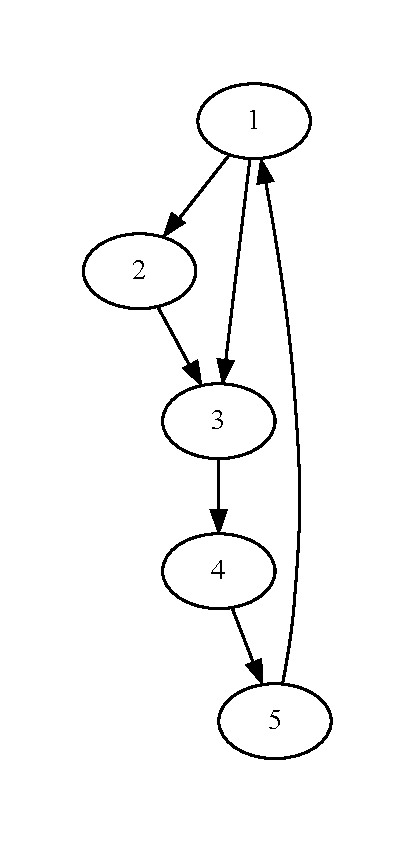
\includegraphics[scale=0.5]{graph1.pdf} \\
graph2.dot: A graph with 10 vertices, with no dead ends nor spider traps. \\
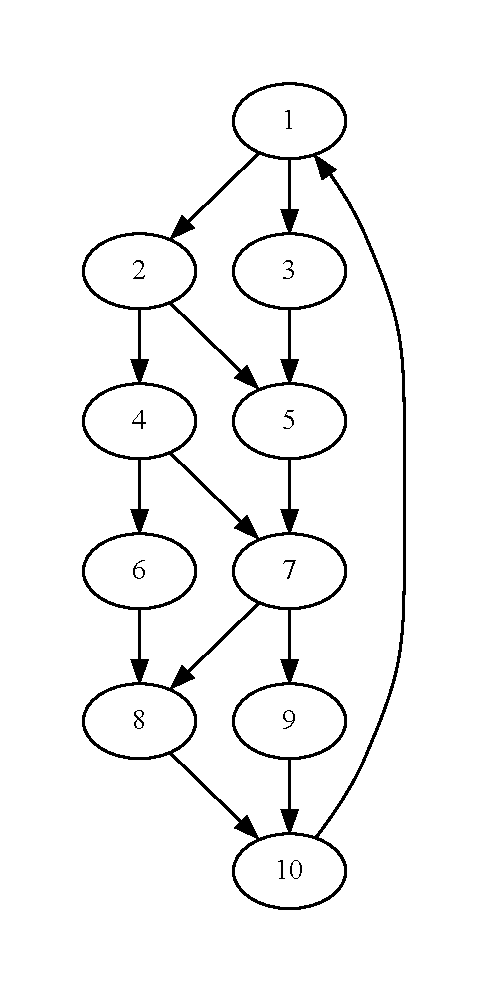
\includegraphics[scale=0.5]{graph2.pdf} \\
graph3.dot: A graph with 10 vertices, with one dead end and no spider traps. \\
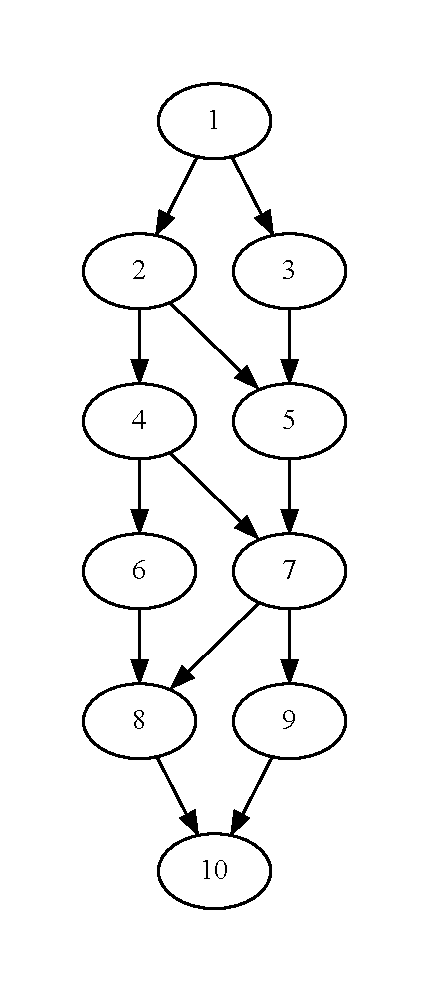
\includegraphics[scale=0.5]{graph3.pdf} \\
graph4.dot: A graph with 10 vertices, with one spider trap and no dead ends. \\
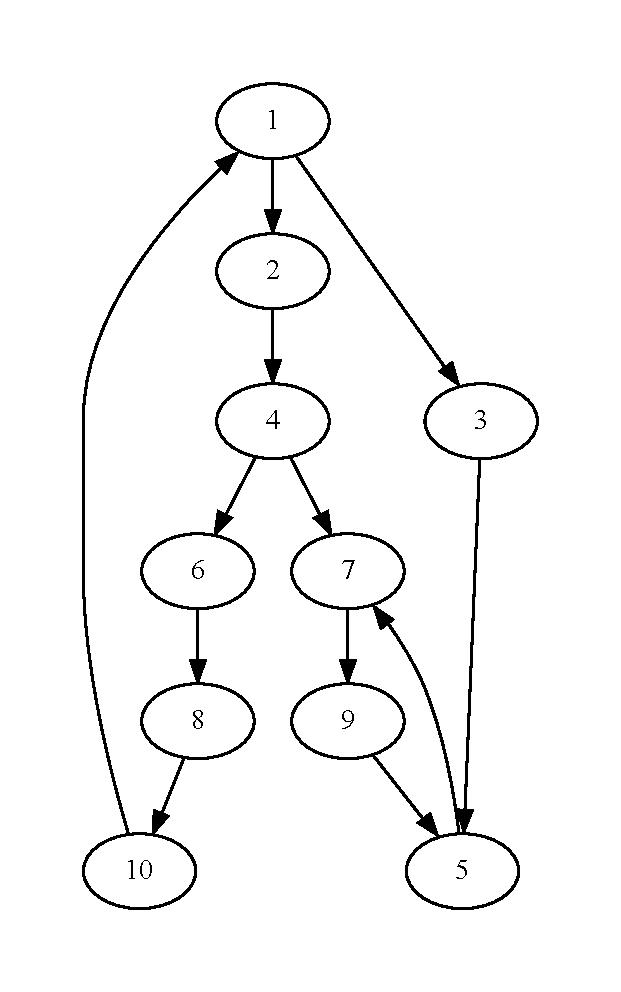
\includegraphics[scale=0.5]{graph4.pdf} \\
graph5.dot: A graph with 50 vertices, which may or may not contain dead ends and/or spider traps. \\
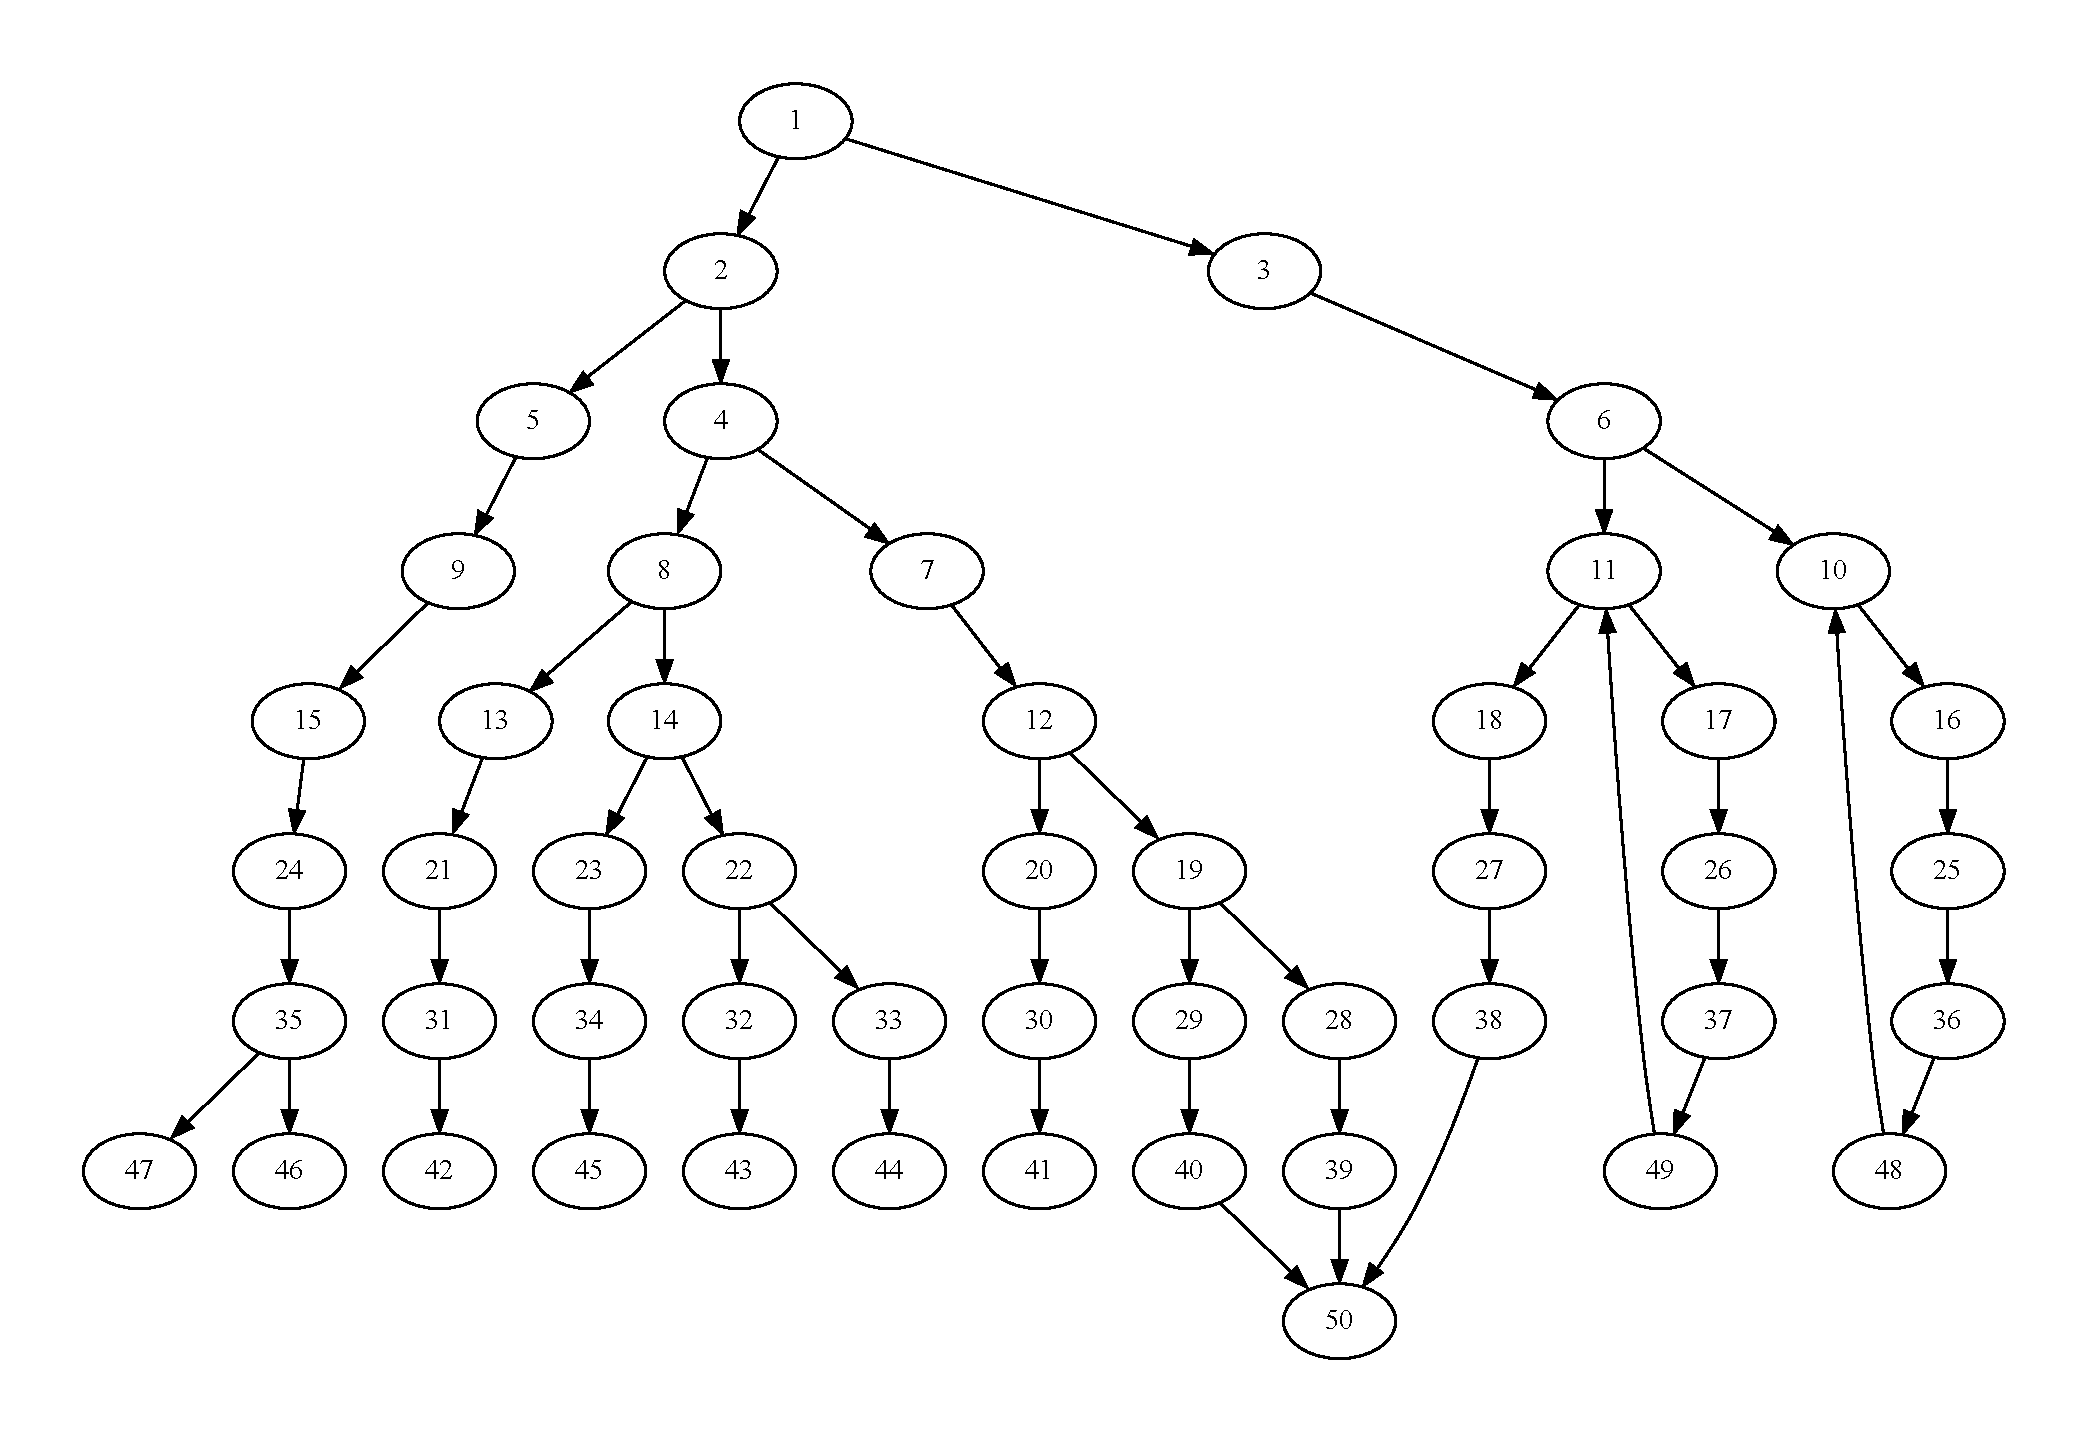
\includegraphics[scale=0.5]{graph5.pdf} \\
\end{center}




\section*{Implementation}
I implemented the page rank algorithm, which ranks the importance of the website pages based on the number of pages/nodes that directly point to the page itself. It works as follows: \\\\
First, I assign a normalized equal rank to every node (that represents a web page) in my graph. Then it enters a while loop, which keeps iterating until the rank for every node stays constant. Inside each iteration, I compute the new rank for each node. I first sum all the ranks coming from its incoming links and multiply the sum by a transition probability. Then, for each node, I also add the leaked PageRank, which is the rank coming from the teleportation of the rest of the graph. Finally, I update the old page rank with the new page rank, and stop when the old page rank and new page rank converge. \\\\
To deal with dead-ends and spider traps, I add the random teleportation feature, meaning when each node distributes its own rank to the nodes the it points to, there is a chance that it doesn't follow those paths and randomly gives its rank to another node in the graph that it doesn't points to, essentially teleport to that node. This ensures that whenever there is a spider trap or dead-end, the rank of those nodes can still teleport out of the structure without being trapped and allow the algorithm to continue.  \\\\
For my algorithm, I set the transition probability to 0.85, which means 85 percent of the time a node will distribute its rank following the outgoing links, and 15 percent of the time it will teleport to another node that it doesn't point to.


\section*{Experiment and Results}

I applied my page rank algorithm to the 5 data sets that I created and ordered the final rank for each node from largest to smallest. \\

For graph1.dot, the final rank for each node is as follows:\\
\begin{center}
\begin{tabular}{ |c|c| } 
 \hline
 vertex & PageRank  \\ 
\hline
 3 & 0.22463635530343473  \\ 
 4 & 0.22094989556193523  \\ 
  5 & 0.21783101930693619  \\ 
   1 & 0.21515524221664378  \\ 
    2 & 0.12142748761105006  \\ 
 \hline
\end{tabular}
\end{center} 

For graph2.dot, the final rank for each node is as follows:\\
\begin{center}
\begin{tabular}{ |c|c| } 
 \hline
 vertex & PageRank  \\ 
\hline
10 & 0.16520479243967118 \\
1 & 0.1554650098593555 \\ 
7 & 0.1366312055323921\\ 
5 & 0.11836760221753825\\ 
8 & 0.10366116779095888\\ 
2 & 0.0810726291902261\\ 
3 & 0.0810726291902261\\ 
9 & 0.07305035272630137\\ 
4 & 0.04945586740584611\\ 
6 & 0.03601874364748461\\ 
 \hline
\end{tabular}
\end{center} 

For graph3.dot, the final rank for each node is as follows:\\
\begin{center}
\begin{tabular}{ |c|c| } 
 \hline
 vertex & PageRank  \\ 
\hline
10 & 0.24688304101855146\\ 
8 & 0.14980639776613824\\ 
7 & 0.14672395472051367\\ 
5 & 0.10137601732339759\\ 
9 & 0.09833938602053334\\ 
6 & 0.06054477233530964\\ 
4 & 0.05778170500222917\\ 
2 & 0.051280088485840966\\ 
3 & 0.051280088485840966\\ 
1 & 0.03598454884164497\\ 
 \hline
\end{tabular}
\end{center} 

For graph4.dot, the final rank for each node is as follows:\\
\begin{center}
\begin{tabular}{ |c|c| } 
 \hline
 vertex & PageRank  \\ 
\hline
7 & 0.23121849548858867\\ 
5 & 0.22947454928190472\\ 
9 & 0.21149478487966536\\ 
1 & 0.06077227061267072\\ 
10 & 0.053849729397685384\\ 
4 & 0.04970398338346545\\ 
8 & 0.045705563997276905\\ 
2 & 0.040828215010385055\\ 
3 & 0.040828215010385055\\ 
6 & 0.036124192937972824\\ 
 \hline
\end{tabular}
\end{center} 

For graph5.dot, the final rank for the top nodes is as follows:\\
\begin{center}
\begin{tabular}{ |c|c| } 
 \hline
 vertex & PageRank  \\ 
\hline
50 & 0.055112666053946824\\ 
10 & 0.05033250898274329\\ 
16 & 0.04880931881362839\\ 
25 & 0.04752539363986613\\ 
36 & 0.046432183653488765\\ 
48 & 0.04549020357345086\\ 
11 & 0.036025238393524686\\ 
49 & 0.028620663256420147\\ 
37 & 0.02657614769054916\\ 
38 & 0.02657614769054916\\ 
 \hline
\end{tabular}
\end{center} 

\section*{Insights and Lessons Learned}
From the experiment results shown above, we can see that when there are no dead ends nor spider traps (graph1.dot), the highest rank tends to go to the node that has the most incoming link, which is node 3 in this case. This makes sense because a web page with more incoming links means more other websites are citing this one, making it more important and credible. This finding is confirmed by graph2.dot, where nodes 10, 1, 7, 5, and 8 have the highest ranks because they have two incoming links (except for node 1, but it also has a high rank because it is the only node 10 is linked to), which is more than the rest of the nodes that only have one incoming link.\\\\
When there is a dead end (graph3.dot), I noticed that the dead end's rank (node 10, rank 0.247) is significantly larger than the rest of the nodes. 
This is because the rank gets trapped inside the dead end since it doesn't have an out-link. However, we are still able to let the rank goes to other nodes through teleportation. \\\\
When there is a spider trap(graph4.dot), I noticed that the majority of the rank is trapped within the spider trap, which is the subgraph formed by nodes 7, 9, and 5. This also makes sense because they are unable to escape except through teleportation. \\\\
Finally, the above insights are again proven by graph5.dot, where nodes 50, 10, 16, and 25 have the highest rank. These are nodes that are either dead ends or within spider traps. \\\\
The most important lesson I learned from this assignment is that teleportation is a solution to dead ends and spider traps. Rather than being trapped within a node or a substructure, rank can escape to other nodes through teleportation, allowing the algorithm to continue. However, spider traps and dead ends still have larger ranks than the rest of the nodes.
\end{document}

